\documentclass[master,14pt,subf,href,colorlinks=true
%,times        % шрифт Times как основной
%,fixint=false % отключить прямые знаки интегралов
]{disser}

\usepackage[utf8]{inputenc}
\usepackage{graphicx}
\usepackage{mathtools}

\usepackage[a4paper, mag=1000, includefoot, left=3cm, right=2cm, top=2cm, bottom=2cm, headsep=1cm, footskip=1cm]{geometry}
\usepackage[T2A]{fontenc}
\usepackage[english,russian]{babel}
\ifpdf\usepackage{epstopdf}\fi

% Номера страниц сверху и по центру
%\def\headfont{\small}
%\pagestyle{headcenter}
%\chapterpagestyle{empty}

% Точка с запятой в качестве разделителя между номерами цитирований
%\setcitestyle{semicolon}

% Использовать полужирное начертание для векторов
\let\vec=\mathbf

% Включать подсекции в оглавление
\setcounter{tocdepth}{2}

\graphicspath{{figure/}}

\begin{document}

\institution{ГОУ ВПО «Московский физико-технический институт (государственный университет)»\\Факультет молекулярной и химической физики\\Кафедра физики высокотемпературных процессов, ОИВТ РАН}
%\\Объединенный институт высоких температур РАН}

% Имя лица, допускающего к защите (зав. кафедрой)
\apname{Фортов В. Е.}

\title{Выпускная квалификационная работа\\[-14pt]на соискание степени\\МАГИСТРА}

\topic{Колебания решетки и динамика дефектов в гамма-уране}

% Автор
\author       {Фиданян Карен Саркисович} % ФИО
\group        {041} % Группа
\coursenum    {03.04.01 } % Номер направления
\course       {Прикладные математика и физика}
\masterprognum{0109104} % Номер магистерской программы
\masterprog   {Молекулярная физика}

% Научный руководитель
\sa      {Стегайлов В. В.}
\sastatus{д.~ф.-м.~н., зав. отд. в ОИВТ РАН}

% Рецензент
%\rev      {}
%\revstatus{}
% Второй рецензент
%\revsnd      {ФИО рецензента}
%\revsndstatus{}

% Консультант
%\con{ФИО консультанта}
%\conspec{вопросам\\охраны труда}
%\constatus{к.~т.~н., доц.}
% Второй консультант
%\consnd{ФИО консультанта}
%\consndspec{экономическим\\вопросам}
%\consndstatus{к.~э.~н., доц.}

% Город и год
\city{Москва}
\date{\number\year}

\maketitle

%%
%% Titlepage in English
%%
%
%\institution{Name of Organization}
%
%% Approved by
%\apname{Professor S.\,S.~Sidorov}
%
%\title{Master's Thesis}
%
%% Topic
%\topic{Dummy Title}
%
%% Author
%\author{Author's Name} % Full Name
%\course{Physics} % Название специальности
%
%\group{} % Study Group
%\masterprog {Title of program}
%
%% Scientific Advisor
%\sa       {I.\,I.~Ivanov}
%\sastatus {Professor}
%
%% Reviewer
%\rev      {P.\,P.~Petrov}
%\revstatus{Associate Professor}
%
%% Consultant
%\con{}
%\conspec{}
%\constatus{}
%
%% City & Year
%\city{Saint Petersburg}
%\date{\number\year}
%
%\maketitle[en]

\tableofcontents

\section{Введение}
Диффузия точечных дефектов определяет скорость самодиффузии, диффузии продуктов деления и прочих включений в ядерном топливе. Она также играет определяющую роль в подвижности дислокаций в кристалле~\cite{dislocation_mobility}.
Понимание кинетики диффузии важно для предсказания эволюции механических и переносных свойств материала.

К сожалению, сущетвует не так много методов для экспериментального изучения диффузии дефектов. Основные причины этого в слабой технике наблюдения на атомных масштабах и большое количество одновременно протекающих процессов, которые трудно различать. Эксперименты проводятся с помощью позитронно-аннигиляционной спектроскопии~\cite{Hehenkamp_experiments_1994, Positron_annihilation_Poland, Positron_annihilation_India, Positron_annihilation_France} при низких температурах и дифференциальной дилатометрии~\cite{Hehenkamp_experiments_1994} при высоких. Но эти методы определяют только концентрацию и имеют низкое пространственное разрешение. И хотя эти методы дают полезную информацию об энергии образования дефектов, они не позволяют определить энергию миграции.

Атомистическое моделирование -- распространенный метод изучения микроскопических свойств твердых тел. Но диффузия дефектов относительно медленный процесс, особенно для квантовых расчетов. Есть успешные попытки моделировать диффузию явно при очень высоких температурах~\cite{Mattsson_DFT_Mo}, но прямое квантовое моделирование слишком вычислительно затратно для ежедневного применения.
В последние годы прогресс в квантовых вычислениях привел к созданию точных межатомных потенциалов для урана~\cite{U_SSS_2012, U_Mo_Xe_2013, U_MEAM_Beeler, U_MEAM_Argentine}, на котором мы сосредоточили наши исследования. Эти модели открыли путь для моделирования объемно-центррованного кубического $\gamma$-урана и дефектов решетки с помощью классической молекулярной динамики. Эти свойства, в свою очередь, могут быть положены в основу метода кинетического Монте-Карло, позволяющего проводить моделирование на временах вплоть до секунд и выше~\cite{kMC_1991}.
На протяжении 20-го века была разработана теория переходного состояния (ТПС) для расчета энергии активации и эффективных частот для активационных процессов в газах и жидкостях~\cite{Eyring}, и позднее для твердых тел, в предположении гармоничности межатомных взаимодействий~\cite{Vineyard, Manley_1960, Glyde_1967}. Эта теория успешно применяется для легких элементов, таких как алюминий, медь и тд.
Однако тяжелые элементы, такие как уран, молибден и им подобные, имеют сложную электронную структуру и фазовую диаграмму. На высоких температурах уран представлен ОЦК-фазой, но при низких температурах и нормальном давлении ОЦК-фаза нестабильна. Это делает применение статических методов предсказания затруднительным. Вдобавок, ангармоничность в ОЦК-металлах становится существенной при относительно низких температурах~\cite{Asker_bcc_Mo_instability,Ozolins_bcc_W_instability}, и гармоническая модель не может описать термодинамику, концентрацию и подвижность дефектов.


В последние годы исследователи активно ищут пути изучения ангармонических свойств кристаллов. Есть очень многообещающие работы по созданию температурно-зависимых эффективных потенциалов~\cite{Hellman_Abrikosov_2013} и методов восстановления ангармонического вклада в энергию из DFT-расчетов при нулевой температуре\cite{Glensk_Breakdown_2014, Glensk_Understanding_anharmonicity_2015}, однако на сегодняшний день нет общепринятой точки зрения по этому вопросу. В то время как авторы предлагают новые методы определения межатомных потенциалов, мы пытаемся решить проблему ангармоничности, пользуясь универсальными EAM потенциалами, которые показали себя достаточно точными.

В предыдущем десятилетии был предложен и разработан метод метадинамики - новый способ изучения поверхности свободной энергии~\cite{Metadynamics_2005, Metadynamics_2006, Metadynamics_2008}. Он позволяет выйти за рамки гармонического приближения и рассчитать температурную зависимость свободной энергии.

В последние годы ученые успешно применяют метадинамику для изучения диффузионных свойств твердых тел~\cite{Aschauer_2009, Kozma_2012, Rabone_2015_1, Rabone_2015_2}.

В разделе \ref{chapter_direct_MD} описано прямое МД-моделирование диффузии, которое мы провели, затем в разделе \ref{chapter_kinetics} мы даем краткий обзор наиболее часто применяемой кинетическо модели для твердых тел -- теории Вайнъярда. В разделе \ref{chapter_frequency} обсуждены специфические трудности, возникающи при моделировании $\gamma$-U при низких и нулевых температурах, и после этого в разделе \ref{chapter_barrier} мы предлагаем путь, как получить параметры для уравнения Аррениуса из NEB- и метадинамических расчетов.

\section{Атомистическая модель}\label{chapter_atomistic_model}
\subsection{Межатомные потенциалы}\label{chapter_potentials}
%Model of atomic interactions is one of the key elements in classical MD calculations. For simulation of metals the most used model is semi-empirical Embedded Atom Model (EAM~\cite{EAM_original}). In this model the potential energy of an atom is given as a sum of pairwise interaction and so-called "embedding energy":
Модель межатомного взаимодействия - один из ключевый элементов в классическом МД-моделировании. Наиболее часто используемая модель для симуляции металлов это полу-эмпирическая Модель погруженного атома (EAM~\cite{EAM_original}). В этом приближении потенциальная энергия атома представляется в виде суммы парного взаимодейстия и так называемой "энергии погружения":
\begin{equation}
U_{i} = U_{i}^{pair} + U_{i}(\rho).
\end{equation}
%\noindent The embedding energy is a function of electron density at the atom position:
\noindent Энергия погружения есть функция электронной плотности в точке, где находится данный атом:
\begin{equation}
U_{i}(\rho) = F_i(\rho_{h,i}),
\end{equation}
%where electron density is a sum of densities from all neighbor atoms:
где электронная плотность вычисляется как сумма плотностей, наведенных всеми окружающими атомами:
\begin{equation}
\rho_{h,i} = \sum_{j (\neq i)} \rho_j(R_{ij}).
\end{equation}
%Functions $\rho(R_{ij})$, $F(\rho)$ and $U^{pair}(R_{ij})$ can be obtained from experimentally measured properties (this method is described in original paper of Daw and Baskes~\cite{EAM_original}), or can be fitted to values of forces acting on atoms in quantum simulations~\cite{Potfit2015}.
Функции $\rho(R_{ij})$, $F(\rho)$ и $U^{pair}(R_{ij})$ могут быть получены из экспериментально измеренных свойств материала (этот метод описан в оригинальной статье Доу и Баскеса~\cite{EAM_original}), или могут быть построены таким образом, чтобы праильно описывать значеня сил, получаемые в квантовых расчетах~\cite{Potfit2015}.
%This model is rather universal and appropriate to simulation of pure metals and alloys. Although there is an evidence, that electronic structure of actinides has the dependence on temperature~\cite{Soderlind_1995}, effective EAM potential, obtained from a representative set of DFT-calculated configurations, gives satisfactory description of the various phases and phase transitions at respective temperatures~\cite{U_SSS_2012}.
Эта модель достаточно универсальна и подходит для описания чистых металлов и сплавов. Хотя есть свидетельства, что электронная структура актинидов имеет существенную зависимость от температуры~\cite{Soderlind_1995}, эффективный EAM-потенциал, полученный из репрезентативного набора конфигураций, обсчитанных с помощью теории функционала плотности (DFT), дает удовлетворительное описание различных фаз и фазовых переходов при соответствующих температурах~\cite{U_SSS_2012}.
%The growth of computer power made possible to build EAM potentials for many different and complicated substances. Thus, last years several models for uranium and its alloys have been made~\cite{U_SSS_2012,U_Mo_Xe_2013,U_MEAM_Beeler, U_MEAM_Argentine, U-Zr,ortho-U}, but not all of them are able to simulate both orthorhombic and bcc phase properly. There are also slight shifts in equilibrium density and other properties, for more details see papers mentioned above.
Рост вычислительной мощности сделал возможным построение EAM потенциалов для множества различных и сложных материалов. Так, в последние несколько лет были созданы модели для урана и его сплавов~\cite{U_SSS_2012,U_Mo_Xe_2013,U_MEAM_Beeler, U_MEAM_Argentine, U-Zr,ortho-U}, но не все они способны описывать и орторомбическую, и ОЦК фазу правильно. Также между ними есть небольшие отличия в равновесной плотности и других свойствах, для более детального рассмотрения рекомендуем указанные выше статьи.


%In this work we use EAM potentials for uranium and molybdenum built in 2012-13~\cite{U_SSS_2012,U_Mo_Xe_2013}. We do not discuss properties of molybdenum in this paper, but we made illustrative comparison of vibrational spectra between stable bcc Mo and instable bcc U. You can find it in supplementary materials.
В данной работе мы использовали EAM потенциалы для урана и молибдена, созданные в 2012-13 годах~\cite{U_SSS_2012,U_Mo_Xe_2013}. Мы не обсждаем свойства молибдена в данной статье, но даем наглядное сравнение свойств колебательных спектров стабильного ОЦК-Mo и нестабильного ОЦК-U в сопутствующих материалах.


\section{Прямое моделирование диффузии}\label{chapter_direct_MD}
%Since there is no experimental data on diffusion of vacancies in $\gamma$-U, a possible way to study microscopic properties of diffusion is direct MD simulation with classic interatomic potentials. At temperatures more than 700 Kelvins the diffusion is fast enough for direct observation in a reasonable time.
Поскольку нет экспериментальных данных по диффузии вакансий в гамма-уране, возможный путь изучения микроскопических свойств диффузии -- прямое МД-моделирование с классическими межатомными потенциалами. При температурах больше 700K диффузия идёт достаточно быстро для прямого наблюдения за разумное вычислительное время.
%The system of $5^3, 7^3$ and $15^3$ unit bcc cells was simulated to assure that effect of size does not change the results critically. To eliminate boundary effects, periodic boundary conditions were used. All simulations were carried out with LAMMPS~\cite{LAMMPS} package. 
Системы из $5^3, 7^3$ и $15^3$ элементарных ОЦК-ячеек были смоделированы чтобы убедиться, что размерные эффекты не меняют результат существенно. Чтобы ликвидировать граничные эффекты, были использованы периодические граничные условия. Всё моделирование было проведено с помощью пакета LAMMPS~\cite{LAMMPS}.
%All calculations were made at constant volume ($a$ = 3.493\r{A}~\cite{U_SSS_2012}) to avoid shifts of the vibrational spectrum and potential landscape.
Всё моделирование проводилось при одном и том же объеме ($a$ = 3.493\r{A}~\cite{U_SSS_2012}), чтобы избежать изменения колебательного спектра и потенциального ландшафта.
%Detection of vacancy was done every 10 fs to be sure that all jumps are resolved. Occurrence of the different types of jumps was analyzed, and domination of the $\left\langle 111\right\rangle$ jumps was proved (more than 95\%, detailed data is given in the supplementary material). Poisson distribution of waiting times between jumps was proved.
Определение положения вакансий производилось через каждые 10 фс для уверенност в том, что все отдельные прыжки различимы. Была проанализирована встречаемость разных типов скачков и подтверждено доминирование прыжков по направлению $\left\langle 111\right\rangle$ (более 95\%, детальные данные даны в сопутствующих материалах). Пуассоновское распределение времен ожидания скачков было подтверждено.
%Typical trajectories of vacancy at different temperatures are shown in figure~\ref{graph_trajectories}.
Типичные траектории вакансии при разных температурах показаны на рисунке~\ref{graph_trajectories}.
\begin{figure}[h]
	\begin{center}
		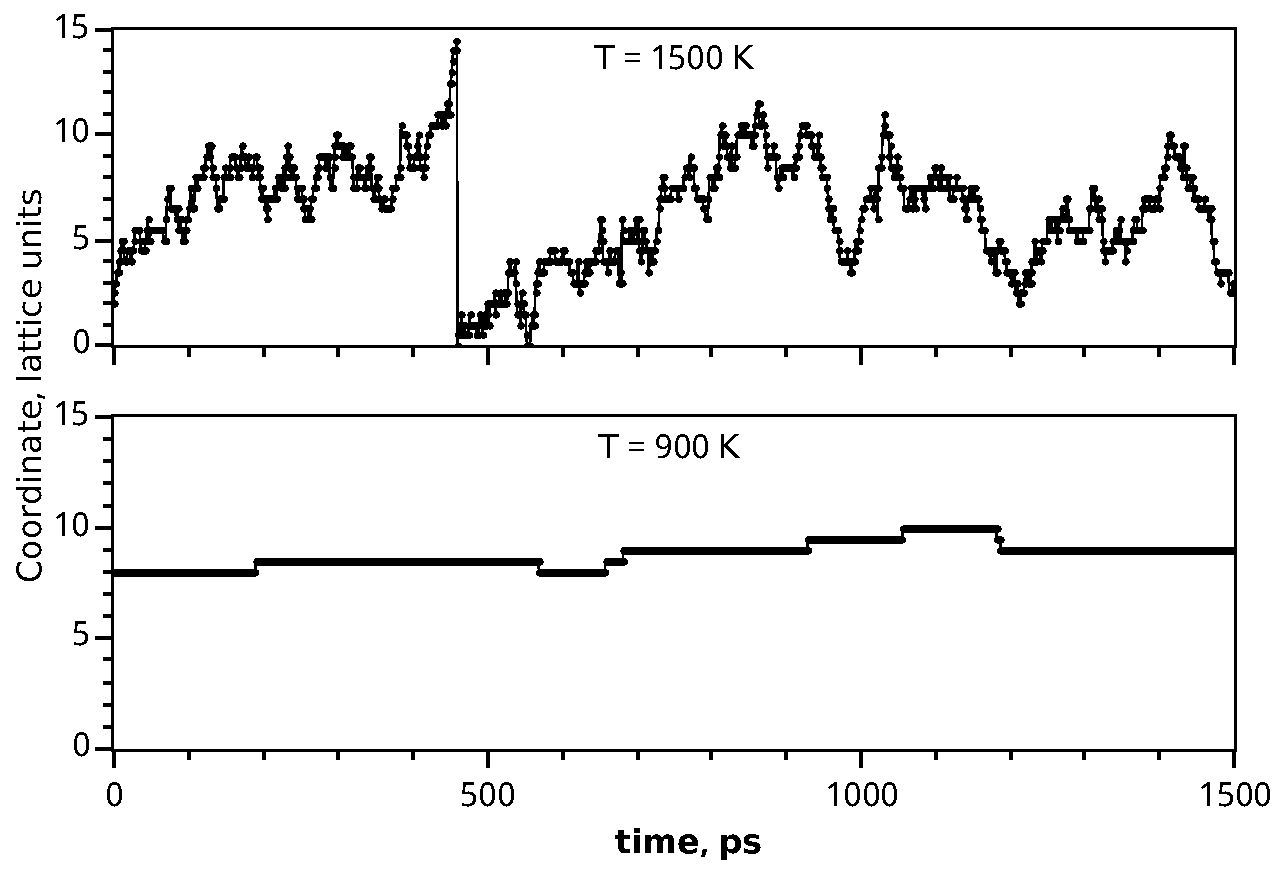
\includegraphics[width=1.\linewidth]{Trajectories.pdf}
	\end{center}
%\caption{Typical trajectories of vacancy at 1500K (top) and 900K (bottom), projected to $x$ axis. On the top trajectory the jump across periodic border is presented.}\label{graph_trajectories}
\caption{Типичные траектории вакансии при 1500K (верхний рисунок) и 900K (нижний), спроектированные на ось $x$. На верхней траектории показан прыжок через периодическую границу.}\label{graph_trajectories}
\end{figure}
%Multiple trajectories of vacancy were analyzed and mean square displacement (MSD) over all trajectories was calculated. The diffusion coefficient was obtained via the Einstein-Smoluchowski equation. Its dependence on temperature is discussed in section \ref{subsection_Metadynamics}. At low temperature it has Arrhenius form, but after 1100 Kelvins diffusivity is lower than Arrhenius equation predicts.
Был проанализирован набор траекторий и построено среднеквадратичное отклонение (СКО) по всем траекториям. Коэффициент дифузии получен через уравнение Эйнштейна-Смолуховского. Его зависимость от температуры обсуждается в разделе \ref{subsection_Metadynamics}. При низких температурах зависимость имеет аррениусовский вид, но начиная с 1100 кельвин подвижность ниже, чем предсказывает уравнение Аррениуса.
\begin{figure}[h]		%MSD
\begin{center}
\begin{minipage}[h]{0.47\linewidth}
\center{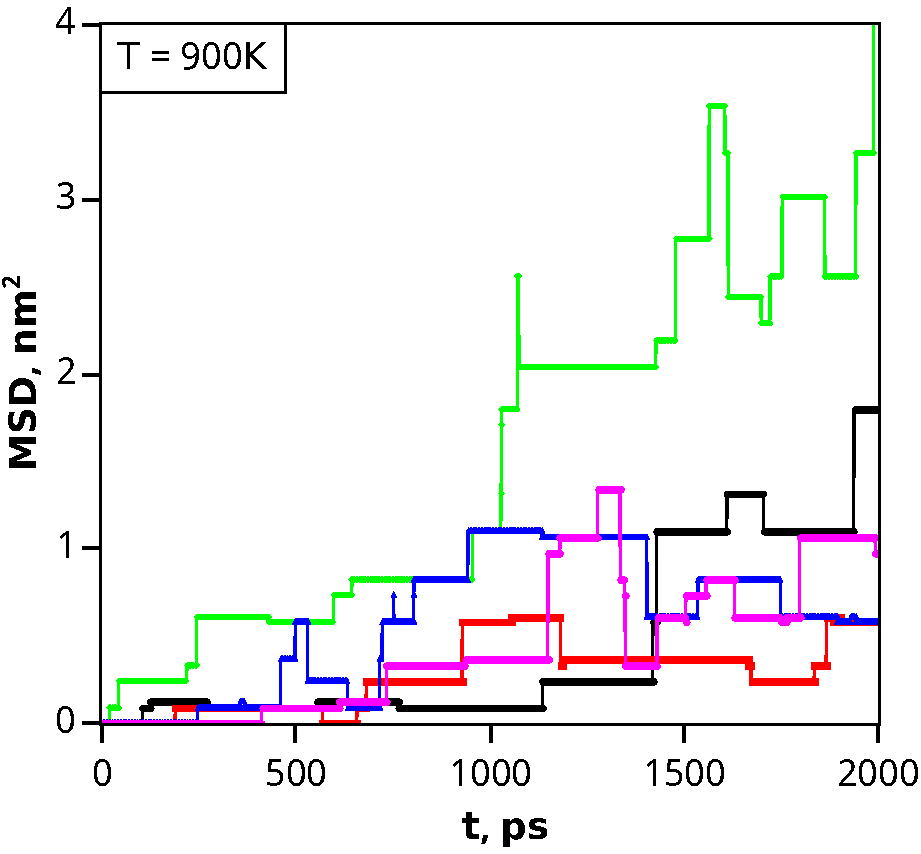
\includegraphics[width=1\linewidth]{MSD_several_900.pdf}} a)
\end{minipage}
\hfill
\begin{minipage}[h]{0.47\linewidth}
\center{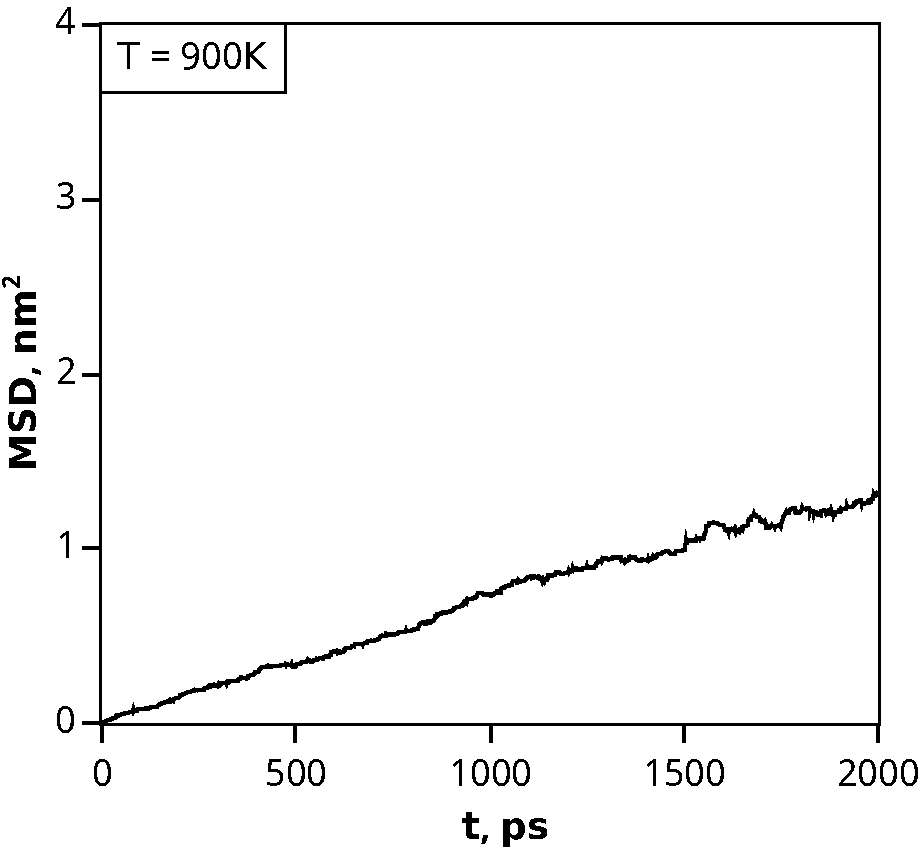
\includegraphics[width=1\linewidth]{MSD_average_900.pdf}} b)
\end{minipage}
\vfill
\begin{minipage}[h]{0.47\linewidth}
\center{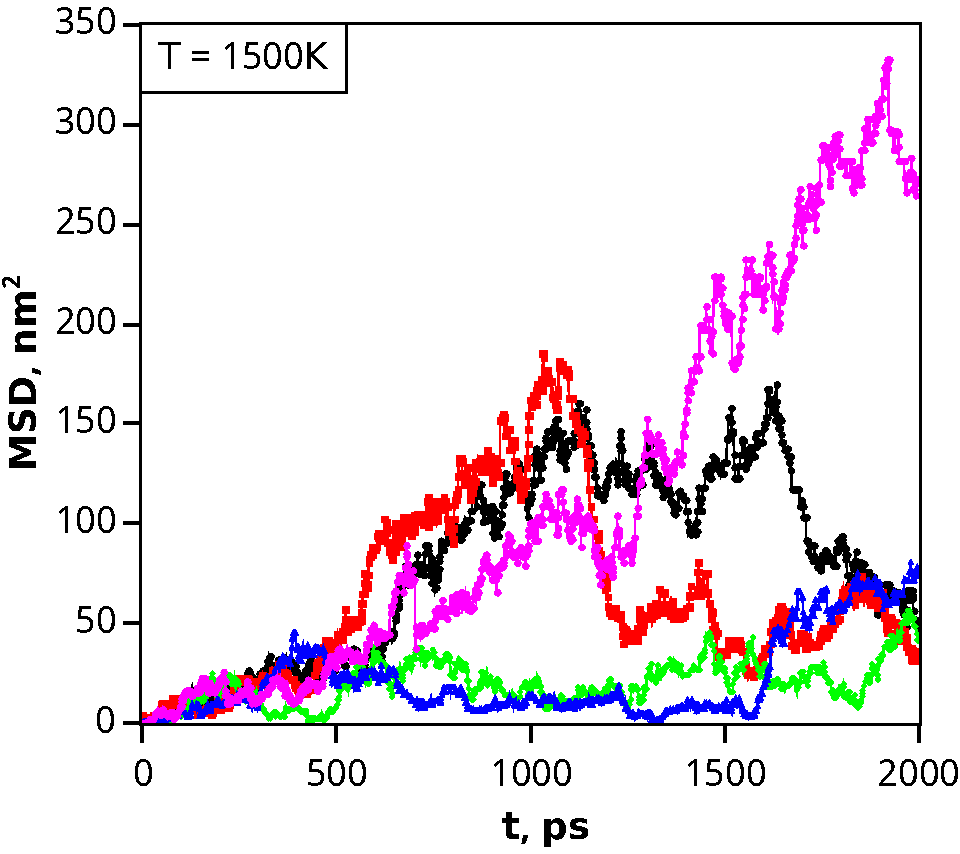
\includegraphics[width=1\linewidth]{MSD_several_1500.pdf}} c)
\end{minipage}
\hfill
\begin{minipage}[h]{0.47\linewidth}
\center{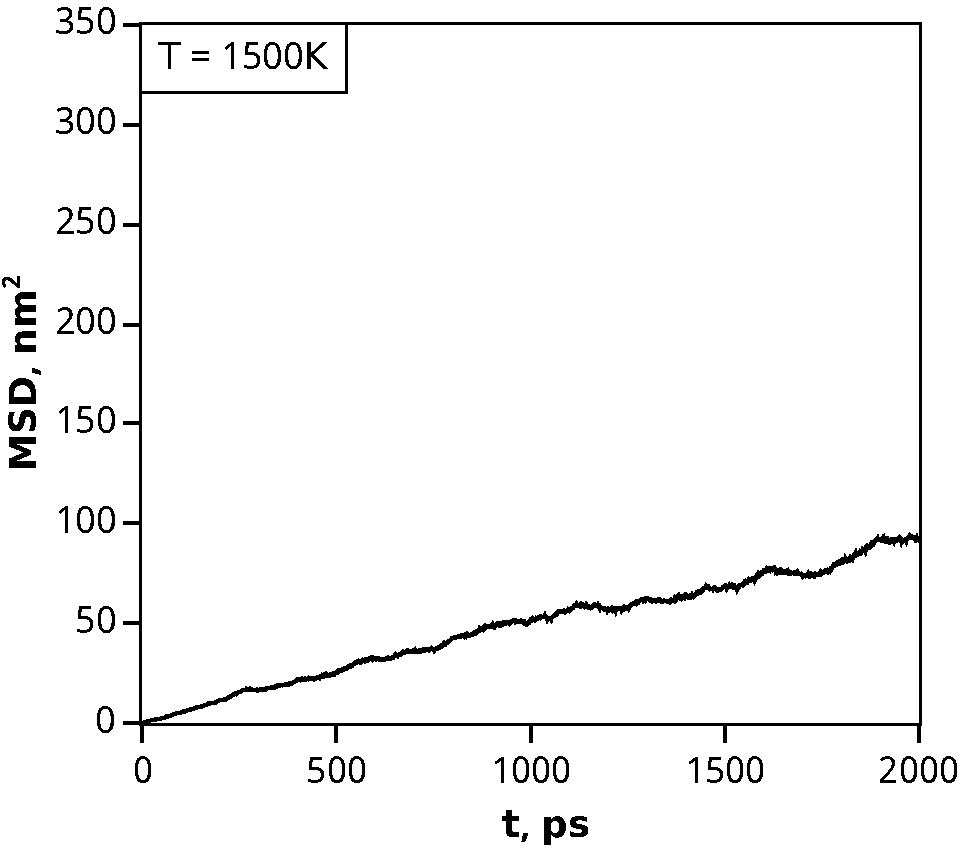
\includegraphics[width=1\linewidth]{MSD_average_1500.pdf}} d)
\end{minipage}
%\caption{Mean Square Displacement for several independent MD trajectories for 900K (a) and 1500K (c). \\MSD averaged over all independent simulations for 900K (b) and 1500K (d).}
\caption{Среднеквадратичное отклонение вакансии от первоначального положения на нескольких нехависимых МД-траекториях для 900K (a) и 1500K (c). \\СКО, усредненное по всем независимым расчетам для 900K (b) и 1500K (d).}
\label{graph_MSD}
\end{center}
\end{figure}
 

\section{Уравнение Аррениуса и теория Вайнъярда}\label{chapter_kinetics}
%Since one should to simulate the evolution of defects on times compared to the period of operation of the reactor materials, native molecular dynamic approach is too demanding. As we want to keep the detailed consideration of atomic processes, a reasonable compromise between specification and computational efficiency is a kinetic approach.
Поскольку необходимо рассчитывать эволюцию дефектов на временах, сопоставимых со сроком эксплуатации реакторных материалов, нативный подход с использованием прямой МД слишком затратен. Если мы хотим сохранить детальное рассмотрение атомных процессов, разумным компромиссом между детализацией и вычислительной эффективностью является кинетический подход.
%Our aim is to build a kinetic model, which could reproduce the results of direct MD with using much less amount of calculations. The model should be applicable both to classic EAM potentials and DFT calculations, it means that simulation of long trajectories is not favorable.
Наша цель -- построить кинетическую модель, которая бы воспроизводила свойства прямого МД моделирования с использованием значительно меньшего количества вычислений. Модель длжна быть прменима как с классическими EAM потенциалами так и с DFT расчетами, это значит, что расчета длинных траекторий лучше избегать.
%In this paper we discuss only vacancies, keeping in mind that same methods can be applied to interstitials too.
В данной статье мы обсуждаем только вакансии, имея в виду, что все те же подходы могут быть применены и к изучению межузельных атомов.

%Diffusion of vacancies can be described via the Transition State Theory (TST)~\cite{TST}. For rare events, system is believed to be in thermodynamic equilibrium almost always. Then the probability of the reaction can be divided into two independent parts: chance that particle reaches the "transition state", i.e. saddle point of the potential surface, and probability that the reacting particle crosses the ridge. 
Диффузия вакансий может быть описана через теорию переходного состояния (ТПС)~\cite{TST}. Для редких событий предполагается, что система большую часть времени пребывает в термодинамическом равновесии. Тогда вероятность события может быть разделена на два независимых сомножителя: вероятность того, что частица достигнет "переходного состояния", т.е. седловой точки на поверхности потенциальной энергии, и вероятность того, что частица пересечет "водораздел".
%Assuming the potential barrier of migration and the vibrational spectrum to be temperature-independent, vacancy jump rate $\Gamma$ should satisfy the Arrhenius equation:
В предположении, что потенциальный барьер и колебательный спектр не зависят от температуры, частота скачков вакансии $\Gamma$ должна удовлетворять уавнению Аррениуса:
\begin{equation}
	\Gamma = \nu  \exp\left[\frac{-E_a}{k_BT} \right],
\end{equation}
%where $E_a$ is the energy of activation of hop from one lattice site to other,
где $E_a$ есть энергия активации скачка из одного узла решетки в другой,
%and $\nu$ is the effective frequency of hop attempts.
а $\nu$ - эффективная частота попыток перескока.

%There are several ways to estimate pre-exponential factor in solids, but most general is a Vineyard theory\cite{Vineyard}. 
Существует несколько способов оценки предэкспоненциального множителя для твердотельных процессов, наиболее общий из них -- теория Вайнъярда\cite{Vineyard}.
%It considers the system of $N$ particles as $3N$-dimensional hyperspace, shown schematically on the figure~\ref{parabolas}a.
Она рассматривает систему из $N$ частиц как $3N$-мерную поверхность потенциальной энергии, показанную схематично на рисунке~\ref{graph_parabolas}a.
%There are two minima $A$, $B$ of potential energy and the $(3N-1)$-dimensional ridge hyperplane $S$ between them. With the assumption that the potential energy is harmonic near the minima and almost harmonic near the saddle point $P$ (i.e. harmonic in $x_{2} \ldots x_{3N}$ subspace, which is orthogonal to the reaction path). 
Есть два минимума потенциальной энергии, $A$ и $B$, и $(3N-1)$-мерная плоскость водораздела $S$ между ними. В предположении, что потенциал гармонический вблизи минимумов и почти гармонический вблизи седлоой точки $P$ (т.е. гармоничен во всем подпространстве $x_{2} \ldots x_{3N}$, которое ортогонально направлению реакции).
%Vineyard showed that jump rate can be written as 
Вайнъярд показал, что частота скачков может быть записанаа как
\begin{equation}\label{Vineyard_first}
	\Gamma = \left( \frac{\prod\limits_{j=1}^{3N} {\tilde{\nu}_j} } {\prod\limits_{j=2}^{3N} {\tilde{\nu}_j'} } \right) \exp\left( - \frac{U(P) - U(A)} {k_BT} \right),
\end{equation}

%\noindent where U is total potential energy, \\$\tilde{\nu}_j$ are all $3N$ normal frequencies of the crystal in minimal state, \\$\tilde{\nu}_j'$ are $3N-1$ frequencies when transiting atom can move only along the hyperplane $S$. 
\noindent где U это полная потенциаьная энергия,\\$\tilde{\nu}_j$ -- все $3N$ нормальные частоты кристалла в положении минимума, \\$\tilde{\nu}_j'$ -- $(3N-1)$ частоты в точке $P$ при условии, что система может двигаться только вдоль гиперплоскости  $S$.

\begin{figure*}[h]	%parabolas
	\begin{center}
		%\begin{minipage}[b]{18pc}
		%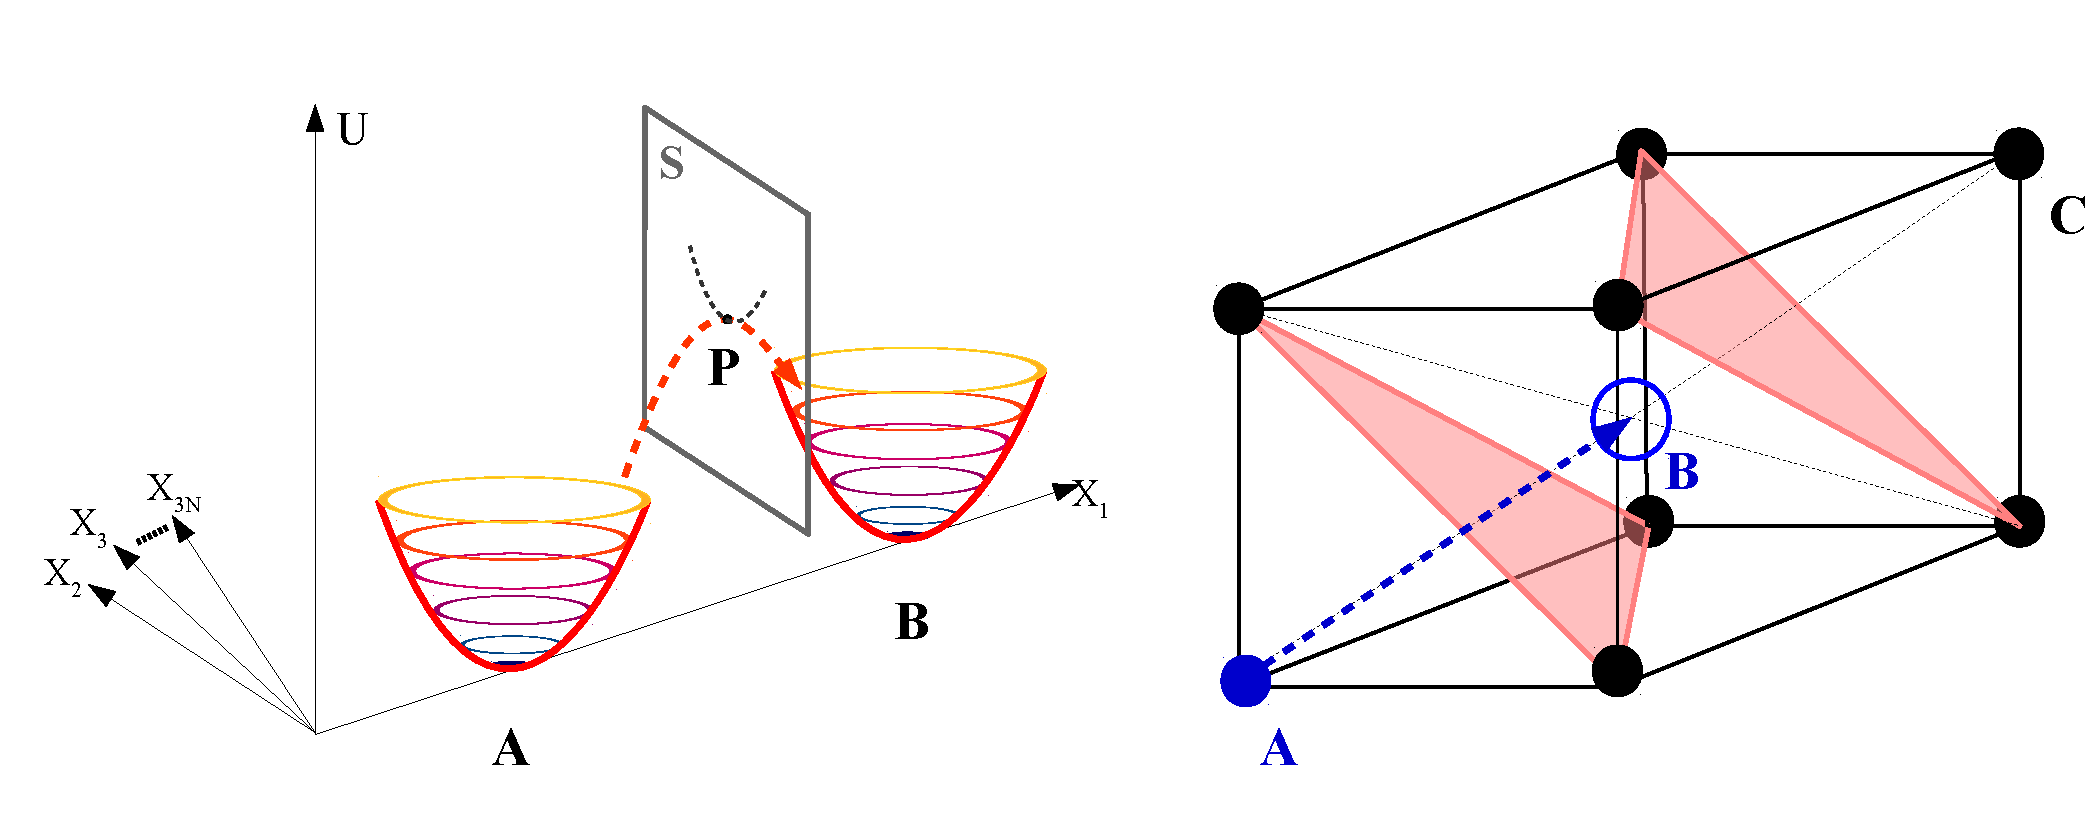
\includegraphics[height=15pc]{Parabolas.pdf} %\hspace{2pc}%
		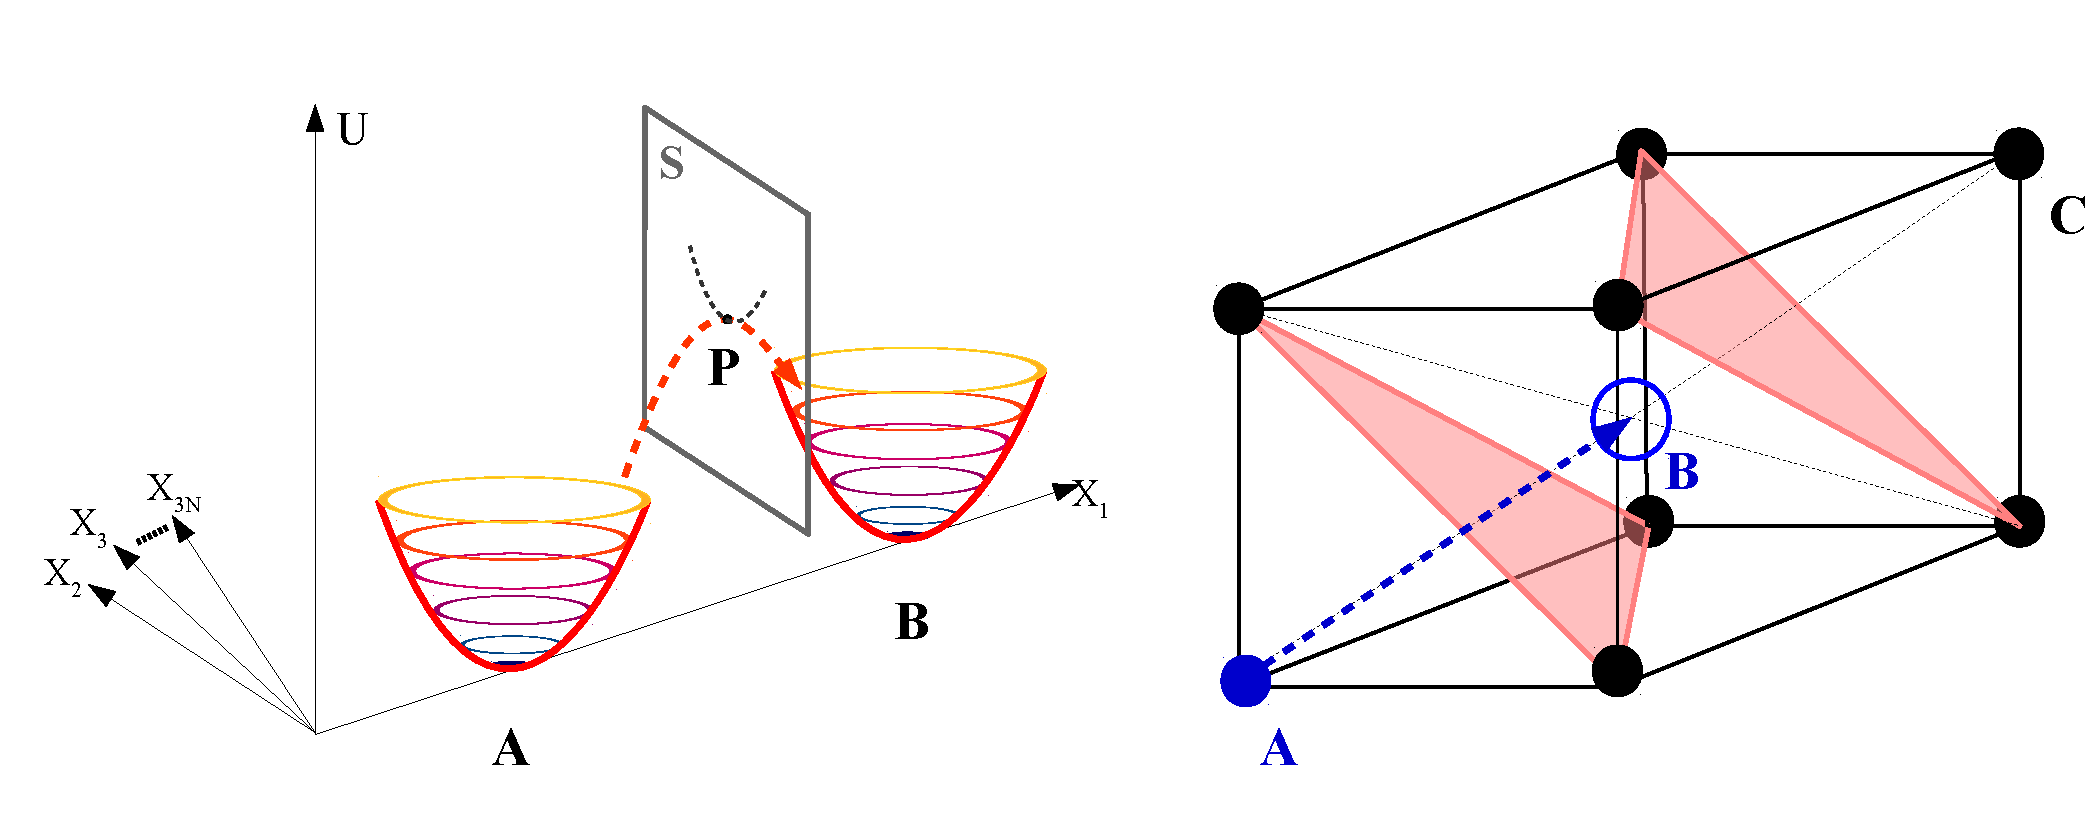
\includegraphics[width=1\linewidth]{Parabolas.pdf} %\hspace{2pc}%
		%\end{minipage}
\caption{\label{graph_parabolas}a) Конфигурационное $3N$-мерное пространство, схематично показывающее два потенциальных минимума системы $A$, $B$ и воображаемую гиперплоскость водораздела $S$, которая разделяет эти минимумы. Приближение Вайнъярда требует, чтобы потенциал в точке $P$ был гармоническим вдоль гиперплоскости $S$.
b)} Прыжок атома в соседний вакантный узел в направлении $\left\langle111\right\rangle$, которое наиболее часто встречается при миграции дефектов в ОЦК-решетке.
	\end{center}
\end{figure*}

%Although Vineyard theory is pretty simple mathematically, its implementation in practice involves difficulties in both finding the energy barrier and calculation of $\tilde{\nu}_j$ and $\tilde{\nu}_j'$. 
Хоя теория Вайнъярда достаточно проста математически, её реализация на практике связана с трудностями как при определении барьера реакции, так и при вычислении $\tilde{\nu}_j$ и $\tilde{\nu}_j'$.
%In the chapter~\ref{chapter_frequency} we review the Vineyard theory for defect migration and then discuss its applicability to bcc lattice of U. We discuss certain peculiarities, which appear because of instability of bcc $\gamma$-phase of uranium at low temperatures.
В разделе~\ref{chapter_frequency} мы рассмотрим теорию Вайнъярда для миграции дефектов и затем обсудим ее применимость к ОЦК-решетке урана. Мы обсудим проблемы, возникающие из-за нестабильности объемно-центрированной кубической $\gamma$-фазы урана при низкой температуре.


\section{Вычисление предэкспоненциального множителя}\label{chapter_frequency}
%As mentioned above, to build Vineyard model we need to calculate normal vibrational modes of the crystal at the equilibrium state for $\nu_j$ and at the saddle point for $\nu_j'$. The straightforward technique to do it is Lattice Dynamics (LD). The idea is to obtain the matrix of second derivatives of potential energy (also known as Hessian matrix) of the studied system~\cite{Landau_1}:
Как уже упоминалось выше, для построения модели Вайнъярда необходимо рассчитать номальный колебательный спектр \{$\nu_j$\} кристалла в положении равновесия и спектр \{$\nu_j'$\} в седловой точке. Естественный способ получения спектра -- динамика решетки (Lattice Dynamics или LD). Идея заключается в получении матрицы вторых производных потенциальной энергии по всевозможным смещениям атомов системы. Эта матрица также известна как матрица Гесса~\cite{Landau_1}:
\begin{equation}
H = \left( \begin{array}{ccc}
\frac{\partial^2 U}{\partial x_1^2} & ... & \frac{\partial^2 U}{\partial x_1 \partial x_{3N}} \\
... & ... & ... \\
\frac{\partial^2 U}{\partial x_{3N} \partial x_1} & ... & \frac{\partial^2 U}{\partial x_{3N}^2}\\ 
\end{array} \right).
\end{equation}

%\noindent Adding masses to the model, we get a dynamical matrix:
\noindent Добавив в модель массы атомов, получаем динамическую матрицу:
\begin{equation}
M = \left( \begin{array}{ccc}
\frac{1}{m_1}\frac{\partial^2 U}{\partial x_1^2} & ... & \frac{1}{\sqrt{m_1}\sqrt{m_{3N}}}\frac{\partial^2 U}{\partial x_1 \partial x_{3N}} \\
... & ... & ... \\
\frac{1}{\sqrt{m_{3N}}\sqrt{m_1}}\frac{\partial^2 U}{\partial x_{3N} \partial x_1} & ... & \frac{1}{m_{3N}}\frac{\partial^2 U}{\partial x_{3N}^2}\\ 
\end{array} \right).
\end{equation}
%Solving the eigenproblem
Решив задачу на собственные значения
\begin{equation} \label{eigenproblem}
M \mathbf{\tilde{x}} = 4\pi^2\tilde{\nu}^2  \mathbf{\tilde{x}},
\end{equation}
%we obtain normal frequencies as eigenvalues of $M$. Eigenvectors $\mathbf{\tilde{x}}$ show which distortion of the lattice corresponds to each frequency. If we calculate normal modes for a large enough system, say, a few thousands of atoms, we get almost continuous density of vibrational states.
мы получаем нормальные частоты матрицы $M$. Собственные векторы $\mathbf{\tilde{x}}$ показывают, какое смещение атомов соответствует каждой частоте. Если мы рассчитаем нормальные моды для достаточно большой системы, скажем, для нескольких тысяч атомов, мы получим почти непрерывную плотность колебательных состояний.

%Normal spectrum for the uranium is shown in figure~\ref{graph_frequency}.
Нормальный спектр для урана показан на рисунке~\ref{graph_frequency}.
%Bcc-U with EAM potential is mechanically unstable at $T=0$, so we see imaginary modes on its spectrum. But  for first-order phase transition the nucleus of the new phase is needed. Due to limited sizes of the simulation area and periodical boundaries, it cannot appear. So one can do a minimization procedure to obtain mechanically stable almost-bcc state. Doing this, we have a different normal spectrum with remarkably smaller imaginary part. Since Vineyard expression needs all frequencies to be real, this spectrum cannot be used for calculation of pre-exponential factor, but it gives relevant data on vibrational properties of real lattice.
ОЦК-U с EAM потенциалом механически неустойчив при $T=0$, поэтому на спектре появляются мнимые моды. Но для фазового перехода первого рода необходим зародыш новой фазы. В силу ограниченных размеров моделируемой области и периодических граничных условий зародыш не может появиться. Поэтому можно провести минимизацию потенциальной энергии и найти близкое к ОЦК, но механически устойчивое состояние. Проделав это, мы получаем другой спектр с заметно меньшей мнимой частью. Поскольку выражение Вайнъярда требует, чтобы все частоты были действительными, этот спектр также не может быть использован для расчета предэкспоненциального члена, но он дает достоверную информацию о колебательных свойствах реальной решетки.

%For comparison you may look at the normal spectrum of the molybdenum, given in supplementary information. Significant difference between the uranium and the molybdenum becomes visible. Bcc phase of molybdenum is stable at zero temperature, so its normal spectrum is fully real. It also means that no additional minimization needed, because bcc lattice sites are absolute minima of the potential energy.
Для сравнения читатель может посмотреть на нормальный спектр молибдена, представленный в сопроводительных данных. Видна существенная разница между ураном и молибденом. ОЦК-фаза молибдена устойчива при нулевой температуре, поэтому его спектр полностью действителен. Это также означает, что никакой дополнительной оптимизации струкуры не требуется, поскольку узлы ОЦК-решетки являются аболютными минимумами потенциальной энергии.
\begin{figure}[h]		%frequencies
%\begin{minipage}[h]{0.47\linewidth}
%\center{\includegraphics[width=1\linewidth]{Mo_static.eps}} a) \\
%\end{minipage}
%\hfill
\begin{center}
\begin{minipage}[h]{.7\linewidth}
\center{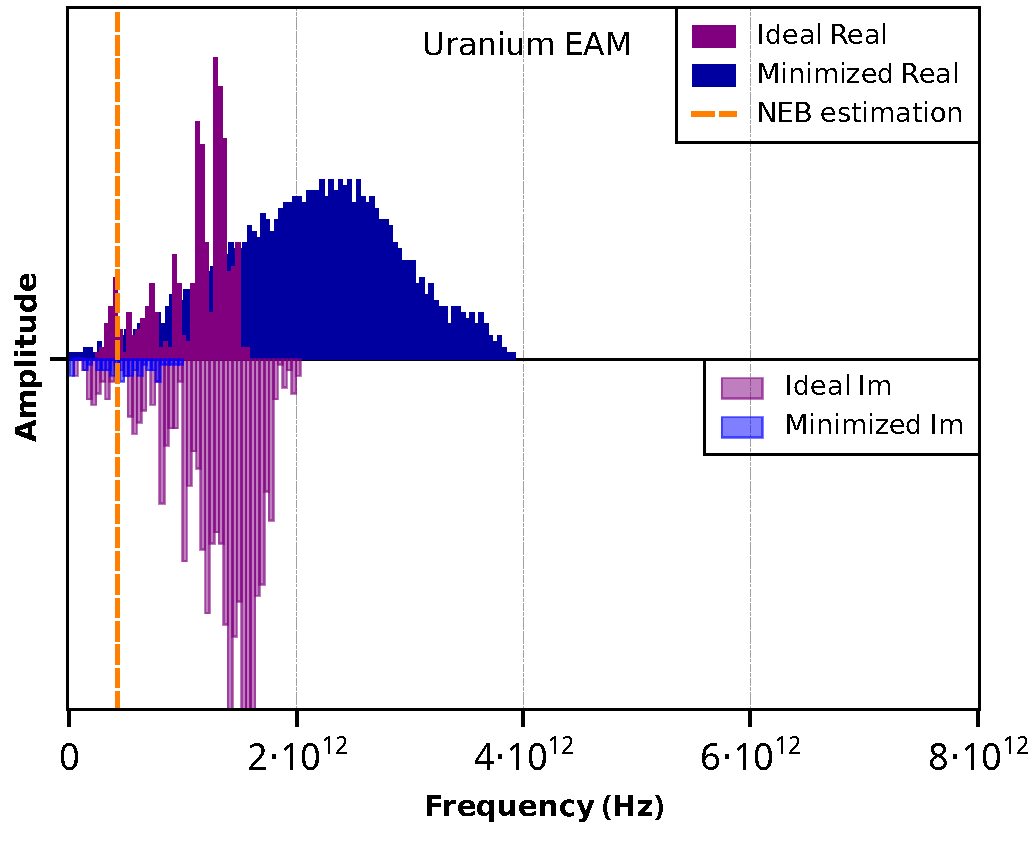
\includegraphics[width=1\linewidth]{U_static.pdf}} a) \\
\end{minipage}
\vfill
%\begin{minipage}[h]{0.47\linewidth}
%\center{\includegraphics[width=1\linewidth]{Mo_dynamic_only.eps}} \\b)
%\end{minipage}
%\hfill
\begin{minipage}[h]{.7\linewidth}
\center{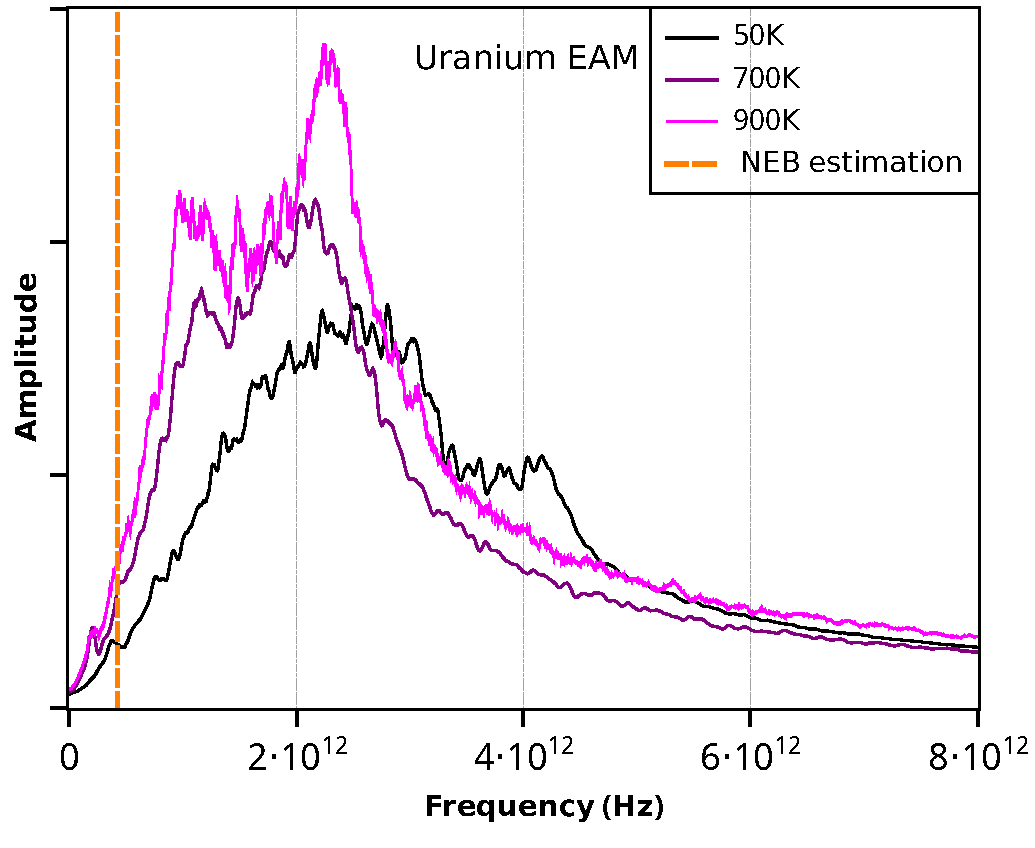
\includegraphics[width=1\linewidth]{U_dynamic_only.pdf}} b) \\
\end{minipage}
%\caption{a) Normal frequency spectra of bcc uranium with EAM potential~\cite{U_SSS_2012}, obtained from static simulation. Instability of bcc phase leads to presence of imaginary frequencies in the cold spectrum. b) The density of vibrational states of bcc U with the EAM potential, obtained via Fourier transform of velocity autocorrelation functions at different temperatures. Orange dashed line represents estimation of frequency factor from curvature of NEB potential.}
\caption{a) Нормальные спектры ОЦК-урана с потенциалом EAM~\cite{U_SSS_2012}, полученные из статических расчетов. Неустойчивость ОЦК-фазы приводит к появлению в спектре мнимых мод. b) Плотность колебательных состояний, полученная с помощью преобразования Фурье автокоррелятора скорости при различных температурах. Оранжевым пунктиром представлена оценка предэкспоненты, сделанная по кривизне потенциала NEB.}
\label{graph_frequency}
\end{center}
\end{figure}


%There is a way how to validate the vibrational spectra obtained from LD. As far as the bcc lattice remains in periodic boundaries with slight distortions only, it is possible to explore its properties with dynamical methods. If we run simulation of a system at finite temperature and calculate velocity autocorrelation function (VACF)
Есть способ проверить колебательне спектры, полученные из статических расчетов (LD). Поскольку в периодических гранусловиях ОЦК-решетка с небольшими искажениями сохраняется, можно изучать её свойства с помощью динамических методов. Если мы запустим расчет траектории системы при конечной температуре и рассчитаем автокорреляционную функцию скорости атомов (АКФС)
\begin{equation*}
	\begin{aligned}
		&g(\tau) = \left\langle \mathbf{v}(0) \cdot \mathbf{v}(\tau)\right\rangle	\\ &(\tau \textnormal{ -- время},  \mathbf{v} \textnormal{  -- скорость})
	\end{aligned}
\end{equation*}
%for a long enough period, its Fourier transform 
для достаточно длинного временного интервала, преобразование Фурье от АКФС
\begin{equation}
F[g](\omega) = \frac{1}{\sqrt{2\pi}}\int \limits_{-\infty}^{\infty} {g(\tau) e^{i\omega \tau} d \tau} 
\end{equation}
%gives us the vibrational density of states (vDoS) for studied system~\cite{Rahman:VACF}. It can be compared to zero temperature LD spectrum. Such comparison is shown at figure~\ref{graph_frequency}.
даст нам плотность колебательных состояний для изучаемой системы~\cite{Rahman:VACF}. Ее можно сравнить с LD спектром при нулевой температуре. Это сравнение показано на рисунке~\ref{graph_frequency}.

\section{Энергетический барьер диффузии}\label{chapter_barrier}
%Another parameter for Arrhenius equation is an activation energy of jumps of vacancy. There are different forms of Arrhenius equation. In most general case Activation energy is a Gibbs energy, but it can be reduced to Helmholtz free energy, because the jump is believed to be fast~\cite{Valikova_2010}, and the change of volume and pressure are local and should not be considered as thermodynamic parameters. Finally, in classic works of Vineyard, Manley and Glyde entropic term is moved to pre-exponential factor and it is considered to be temperature independent, so only the potential energy remains in the exponent~\cite{Vineyard,Manley_1960,Glyde_1967}.
Второй параметр для уравнения Аррениуса -- энергия активации скачка вакансии. Есть разные формы записи уравнения Аррениуса. В наиболее общем виде энергия активации есть энергия Гиббса, но в нашем случае она может быть упрощена до свободной энергии Гельмгольца, поскольку прыжки считаются быстрыми~\cite{Valikova_2010}, и изменение объема и давления в системе являются локальными и не могут рассматриваться как термодинамические величины. Наконец, в классических работах Вайнъярда, Мэнли и Глайда энтропийный член переносится в предэкспоненциальный фактор, так что под экспонентой остается только потенциальная энергия~\cite{Vineyard,Manley_1960,Glyde_1967}.

\subsection{Метод ``Nudged Elastic Band''}
%There is well-known technique to obtain the minimal energy path (MEP) between two minimal states from molecular static simulations. It is so-called Nudged Elastic Band method.
Для поиска путей наименьшей энергии (Minimal Energy Path или MEP) между двумя состояниями-минимумами существует хорошо известный статический метод. Это так называемый ``метод упругой ленты'' (``Nudged Elastic Band'' или NEB).
%The key idea of NEB is simultaneous run of many parallel replicas of the same system, and addition of artificial "forces" between these replicas to make the systems lay along the MEP between two predefined states. When this chain of states takes his place, the second procedure starts for more precise evaluation of the height of the barrier. For the replica with higher potential energy forces along MEP are reversed, and this system "climbs" to the saddle point of MEP. For detailed description of the NEB see papers of G. Henkelman, G. Mills and H. J\'onsson~\cite{NEB_1994, NEB_1995, CI_NEB_2000}.
Основная идея метода NEB заключается в параллельном моделировании нескольких копий одной и той же изучаемой системы, в которых добавлены искуственные ``силы'', связывающие эти копии между собой. Эти силы заставляют копии системы выстраиваться вдоль пути наименьшей энергии между двумя наперед заданными состояниями. Когда эта цепочка располагается вдоль MEP, начинается вторая фаза для уточнения высоты барьера. Для копии с наибольшей потенциальной энергией компоненты сил вдоль MEP инвертируются, и система ``вскарабкивается'' на седловую точку реакции. Для более детального описания см. статьи Г. Хенкельмана, Г. Миллса и Х. Йонссона~\cite{NEB_1994, NEB_1995, CI_NEB_2000}.
%However, there is a problem linked with applying of static methods to bcc uranium.
Однако, применение этого метода для $\gamma$-U наталкивается на проблему.
%The problem is instability of $\gamma$-U lattice at low temperature. Attempts to define completely minimized initial and final states for NEB lead to random displacement of atoms, artificial asymmetry of barrier and nonphysical contributions to barrier from environment atoms. To overcome these problems we used NEB between two quasistable ideal lattices with the vacancy in different sites. We believe that this approach makes sense if we are interested in high temperature processes, occurring in stable bcc phase.
Проблема в неустойчивости решетки гамма-урана при нулевой тепературе. Попытки задать полностью минимизированное начальное и конечное состояния приводят к случайным смещениям атомов, искусственной ассиметрии барьера и нефизичному вкладу в величину барьера от окружающих вакансию атомов. Чтобы преодолеть эти проблемы, мы запускали расчеты NEB между двумя квази-устойчивыми идеальными решетками с различным положением вакансии. Мы считаем, что такой подход оправдан, поскольку интересующий нас процесс происходит при высоких температурах, на которых EAM потенциал дает устойчивую ОЦК-фазу.

%In case of single atomic jumps, the pre-exponential factor for Arrhenius expression also may be roughly estimated in NEB framework. If one calculate the curvature of potential well near the minimal point, it gives the effective frequency $\nu^\mathrm{NEB}$ along the direction of jump. The physical meaning of this frequency is explained in the work of Vineyard\cite{Vineyard}. The pre-exponential factor from equation~\ref{Vineyard_first} can be divided in two parts:
В случае одиночного скачка атома предэкспоненциальный член в выражении Аррениуса также может быть оценен в контексте NEB. Если рассчитать кривизну потенциала вдоль MEP вблизи точки минимума, эта величина даст эффективную частоту $\nu^\mathrm{NEB}$ вдоль направления скачка. Физически смысл этой частоты объяснен в работе Вайнъярда\cite{Vineyard}. Предэкспоненциальный член может быть разделен на две части:
\begin{equation}
	\left( \frac{\prod\limits_{j=1}^{3N} {\tilde{\nu}_j} } {\prod\limits_{j=2}^{3N} {\tilde{\nu}_j'} } \right) = 
	\left( \frac{\prod\limits_{j=2}^{3N} {\tilde{\nu}_j} } {\prod\limits_{j=2}^{3N} {\tilde{\nu}_j'} } \right) \cdot \tilde{\nu}^\mathrm{A}_1 = \exp{\left(\frac{\Delta S}{k_B}\right)}\cdot \tilde{\nu}^\mathrm{A}_1,
\end{equation}
%where $\tilde{\nu}^\mathrm{A}_1$ is exactly equal to $\nu^\mathrm{NEB}$.
где $\tilde{\nu}^\mathrm{A}_1$ в точности равна $\nu^\mathrm{NEB}$.

%\noindent Resulting frequency for $\left\langle 111\right\rangle$ direction is $4.28 \cdot 10^{11}$ Hz. 
Полученная нами частота для скачка в направлении $\left\langle 111\right\rangle$ равна $4.28 \cdot 10^{11}$ Гц.
%It is less than most of other frequencies, and there is an experimental work where such softening is also observed and associated with high diffusion rate~\cite{BCC_Soft_Phonons}.
Это меньше большинства частот в кристалле, и есть экспериментальная работа, в которой показано, что подобное смягчение характерно для многих ОЦК-металлов и коррелирует с высоким коэффициентом диффузии~\cite{BCC_Soft_Phonons}.

%Results of NEB calculation for different vacancy jumps in bcc U are shown in figure~\ref{graph_NEB_parabolas}. Since the barrier along $\left\langle 111\right\rangle$ is lower than others, we concentrate on this mechanism in further research. Direct MD also shows that other directions may be neglected in comparison with $\left\langle 111\right\rangle$ jumps.
Результаты NEB для различных направлений скачка вакансии в ОЦК-U показаны на рисунке~\ref{graph_NEB_parabolas}. Поскольку барьер вдоль $\left\langle 111\right\rangle$ ниже, чем остальные, мы сконцентрировались на этом механизме в наших последующих исследованиях. Прямое МД-моделирование такде показывает, что скачки по остальным направлениям вносят пренебрежимо малый вклад по сравнению с $\left\langle 111\right\rangle$.
\begin{figure}[h]
\begin{center}
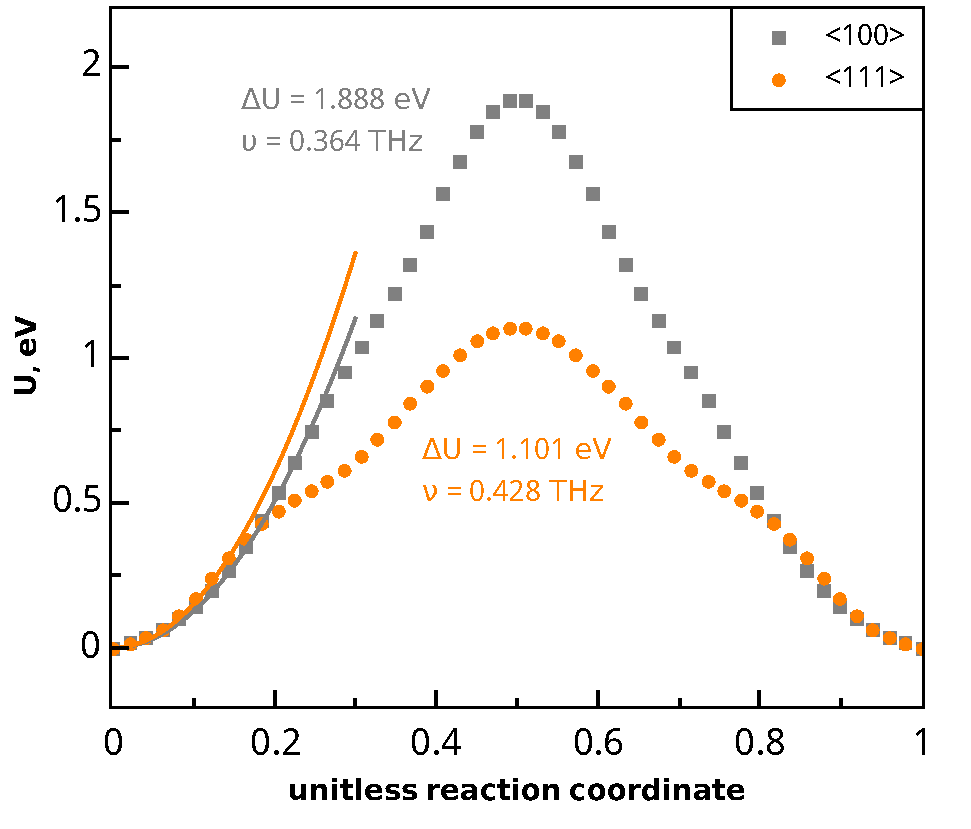
\includegraphics[width=.7\linewidth]{NEB_parabolas.pdf}
\end{center}
%\caption{\label{graph_NEB_parabolas} Results of Nudged Elastic Band simulations for vacancy hops along $\left\langle 111\right\rangle$ and $\left\langle 100\right\rangle$ lattice directions. The curvature near the minimal point gives an estimation for the Einstein frequency for migrating atom. The horizontal axis represents the dimensionless reaction coordinate.}
\caption{\label{graph_NEB_parabolas} Результаты моделирования методом Nudged Elastic Band для скачков вакансии вдоль кристаллографических направлений $\left\langle 111\right\rangle$ и $\left\langle 100\right\rangle$. Кривизна потенциала вблизи точки минимума дает оценку на частоты колебаний для перескакивающего атома. По горизонтальной оси отложена безразмерная координата реакции.}
\end{figure}

%However, the height of the potential barrier and effective frequency, obtained with NEB, cannot describe the results of direct MD simulation which we carried out. NEB cannot describe the slowdown of diffusion at high temperature (see figure~\ref{graph_MSD}). 
Однако высота барьера и эффективная частота, полученные методом NEB, не могут описать результаты прямого МД-моделирования, которое мы провели ранее. NEB не может описать отклонение от закона Аррениуса при высоких температурах (см. рисунок~\ref{graph_MSD}).
%Attempts to measure the temperature dependence of activation energy are mentioned in literature. Thus, authors obtained this dependence for different Lennard-Jones materials~\cite{De_Lorenzi_1987,Sato_2010}. But today there is no generally accepted way how to do it properly.
В литературе встречаются попытки измерить температурную зависимость энергии активации. Так, авторы получили эту зависимость для различных потенциалов Леннард-Джонса~\cite{De_Lorenzi_1987,Sato_2010}. Но на сегодняшний день нет общепринятого подхода к этой проблеме.
%We made finite temperature estimations of activation energy via the metadynamics method, described in the next paragraph.
Мы сделали оценки энергии активации для конечных температур с помощью метода метадинамики, описанного в разделе\ref{subsection_Metadynamics}.

\subsection{Метадинамика}\label{subsection_Metadynamics}
%Metadynamics is a relatively new technique of enhanced sampling~\cite{Metadynamics_2005,Metadynamics_2006,Metadynamics_2008}. It restores the free energy surface (FES) of the studied system via defining a set of collective variables (CVs) and runs biased dynamics with the history-dependent potential:
Метадинамика представляет собой относительно новый метод ускоренного исследования конфигурационного пространства~\cite{Metadynamics_2005,Metadynamics_2006,Metadynamics_2008}. Он восстанавливает поверхность свободной энергии (ПСЭ) иследуемой системы путем задания некоторого набора обобщенных переменных и запуска в них динамики с потенциалом, зависящим от предыстории:
\begin{equation}
V_G(S(x), t) = w \sum\limits_{\mathclap{\substack{t' = \tau_G, 2\tau_G,..., \\ t' < t}}} exp \left( - \frac{\left(S(x) - s(t')\right)^2}{2\delta s^2}\right),
\end{equation}
%where $s(t) = S(x(t))$ is the value taken by the CV at time $t$. \\ Three parameters are needed to define the $V_G$ :\\
%(i) the Gaussian weight $w$\\
%(ii) the Gaussian width $\delta s$\\
%(iii) the frequency $\tau_G$ at which the Gaussians are added to the potential.
где  $s(t) = S(x(t))$ -- значение обобщенной переемнной в момент времени $t$. \\ Для задания потенциала $V_G$ необходиы три параметра:\\
(i) высота гауссианы $w$\\
(ii) ширина гауссианы $\delta s$\\
(iii) частота $\tau_G$, с которой гауссианы добавляются к потенциалу.

%After some time additional potential "fills" the potential well and the system starts to explore new regions of the configuration space. Unlike NEB and other static methods, metadynamics is not restricted by harmonic approximation and can explicitly give the information about dynamics of a studied system at high temperatures.
Через некоторое время дополнительный потенциал ``наполняет'' потенциальную яму, и система начинает исследовать новые участки конфигурационного пространства. В отличие от NEB и других статических методов, метадинамика не ограничена гармоническим приближением и может в явном виде давать информацию о динамике системы при высоких температурах.


%Metadynamic simulations were carried out with LAMMPS-compatible package COLVARS~\cite{COLVARS}. For describing the process we chose the distance between two opposite neighbors of vacancy as a CV. At figure~\ref{graph_parabolas} it is the distance between atoms A and C.
Метадинамическое моделирование проводилось с помощью LAMMPS-совместимого пакета COLVARS~\cite{COLVARS}. Для описания процесса в качестве обобщенной координаты было выбрано расстояние между двумя противостоящими соседями вакансии. На рисунке~\ref{graph_parabolas} это расстояние между атомами A и C.
%As far as vacancy in bcc lattice has 4 pairs of $\left\langle 111\right\rangle$ neighbors, we could take 4 CVs, but their cross-interaction would lead to softening of the environing potential for each of them, making diffusive barrier lower. So we set only one CV for metadynamics, but all the rest were under observation to filter out their spontaneous transitions. 
Поскольку вакансия в ОЦК-решетке имеет 4 пары $\left\langle 111\right\rangle$-соседей, мы могли бы взять 4 обобщенных координаты, но их перекрестное взаимодействие приводило бы к нефизичному смягчению общего потенциала для каждой из них, что сделало бы барьер диффузии ниже. Поэтому мы задали лишь одну из них в качестве метадинамической координаты, но вели наблюдение за всеми, чтобы исключить спонтанные переходы по остальным направлениям.

%Tests of accuracy of the method give interesting results (figure~\ref{graph_MetaD_freq}). Measured barrier strongly depends on the frequency $\tau_G$ of modification of the metadynamic potential. The choice of correct $\tau_G$ is a topic for a discussion.
Исследования точности метода дали интересные результаты (рисунок~\ref{graph_MetaD_freq}). Наблюдаемый барьер сильно зависит от частоты $\tau_G$, с которой обновляется метадинамический потенциал. Выбор корректного значения  $\tau_G$ -- дискуссионный вопрос.
%There are two limits in figure~\ref{graph_MetaD_freq}: right edge corresponds to almost unbiased dynamics, where transitions of defect occur spontaneously and metadynamic potential at the moment of transition is still almost zero; left edge corresponds to fast modification of the potential, giving the minimal estimate of $TS$ term, or the maximal estimate of free energy $\Delta F$. At low temperatures $TS \to 0$, and we see good agreement with the static NEB calculation. Based on these considerations we used "fast" limit in further work.
На рисунке~\ref{graph_MetaD_freq} есть два предельных случая: правый край соответствует практически не измененной динамике, когда переходы происходят спонтанно и метадинамический потенциал в момент перехода еще практически нулевой; левый край соответствует очень быстрому изменению потенциала, которое дает минимальную оценку на член $TS$, или максимальную оценку свободной энергии $\Delta F$. При низких температурах $TS \to 0$, и мы видим хорошее согласие со статическими вычислениями методом NEB. Основываясь на этом, мы использовали в дальнейшей работе ``быстрый'' предел.

%U. Aschauer with coauthors in their work~\cite{Aschauer_2009} noticed that the temperature dependence of diffusion barriers is nonlinear in some cases. In our measures for $\gamma$-U this nonlinearity is pronounced, and we believe that it explains the deviation from Arrhenius equation for diffusion of vacancies, which is clearly visible at figure~\ref{graph_MSD}a.
У. Ашауэр с соавторами в работе~\cite{Aschauer_2009} отмечают, что тепературная зависимость барьеров диффузии в некоторых случаях нелинейная. В наших измерениях для $\gamma$-U эта нелинейность носит ярко выраженный характер, и мы считае, что это объясняет отклонение скорости диффузии вакансий от закона Аррениуса которое хорошо видно на рисунке~\ref{graph_MSD}a.

%FES averaged over several runs are shown in figure~\ref{graph_MetaD_FES}, and temperature dependence of $\Delta F$ is given in figure~\ref{graph_MSD}b.
Поверхности свободной энергии, усредненные по нескольким независимым расчетам, показаны на рисунке~\ref{graph_MetaD_FES}, а температурная зависимость $\Delta F$ дана на графике~\ref{graph_MSD}b.

\begin{figure}[h]	%graph_MetaD_freq
\begin{center}
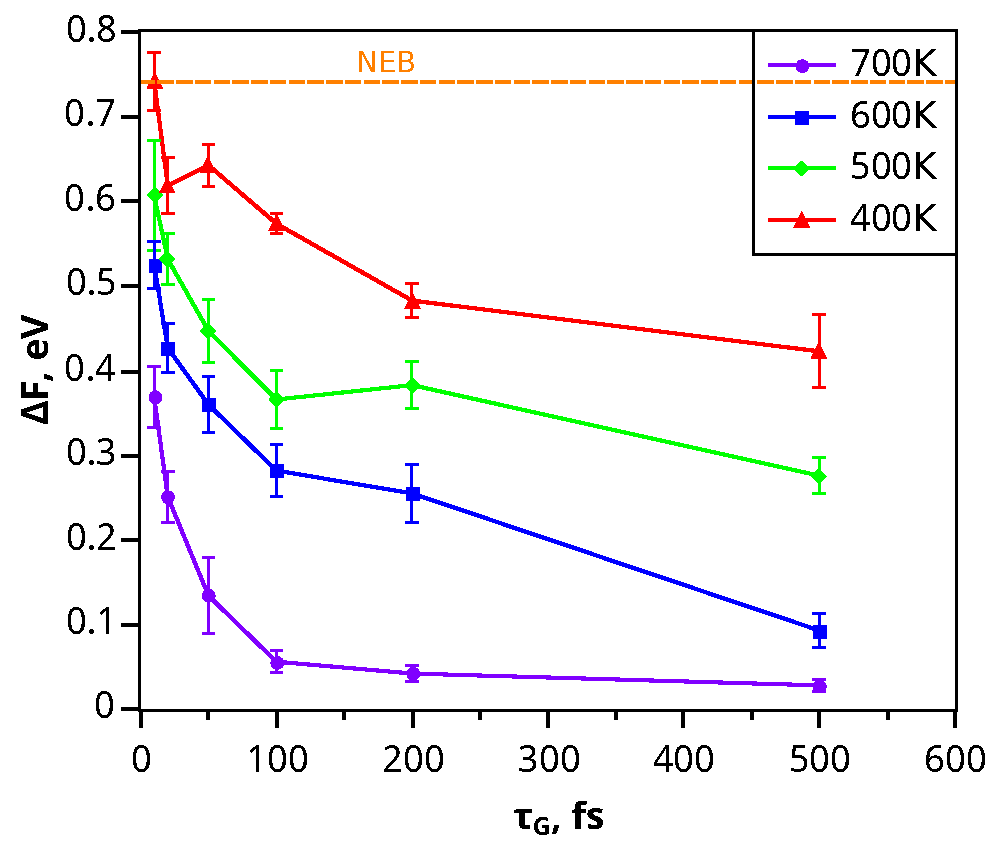
\includegraphics[width=.7\linewidth]{W_T_freq.pdf}
\end{center}
%\caption{\label{graph_MetaD_freq} Results of metadynamic simulation for vacancy hops along $\left\langle 111\right\rangle$ direction at different temperatures and frequency $\tau_G$, at which the Gaussians are added to the potential. This simulation was done for lattice constant $a = 3.54$ \r{A}, so here are different value of NEB barrier, but the general trend is the same. Metadynamic parameters are: $w$ = $2\times10^{-4}$ eV, $\delta s$ = 0.2 \r{A}.}
\caption{\label{graph_MetaD_freq} Результаты метадинамического моделирования для скачков вакансии вдоль направления $\left\langle 111\right\rangle$ при различных температурах и частоте $\tau_G$, с которой к потенциалу добавляются гауссианы. Этот расчет был поведен для постоянной решетки $a = 3.54$ \r{A}, поэтому значение барьера здесь отличается, однако общая зависимость такая же. Метадинамические параметры расчета: $w$ = $2\times10^{-4}$ eV, $\delta s$ = 0.2 \r{A}.}
\end{figure}

\begin{figure}[h]	%graph_MetaD_FES
\begin{center}
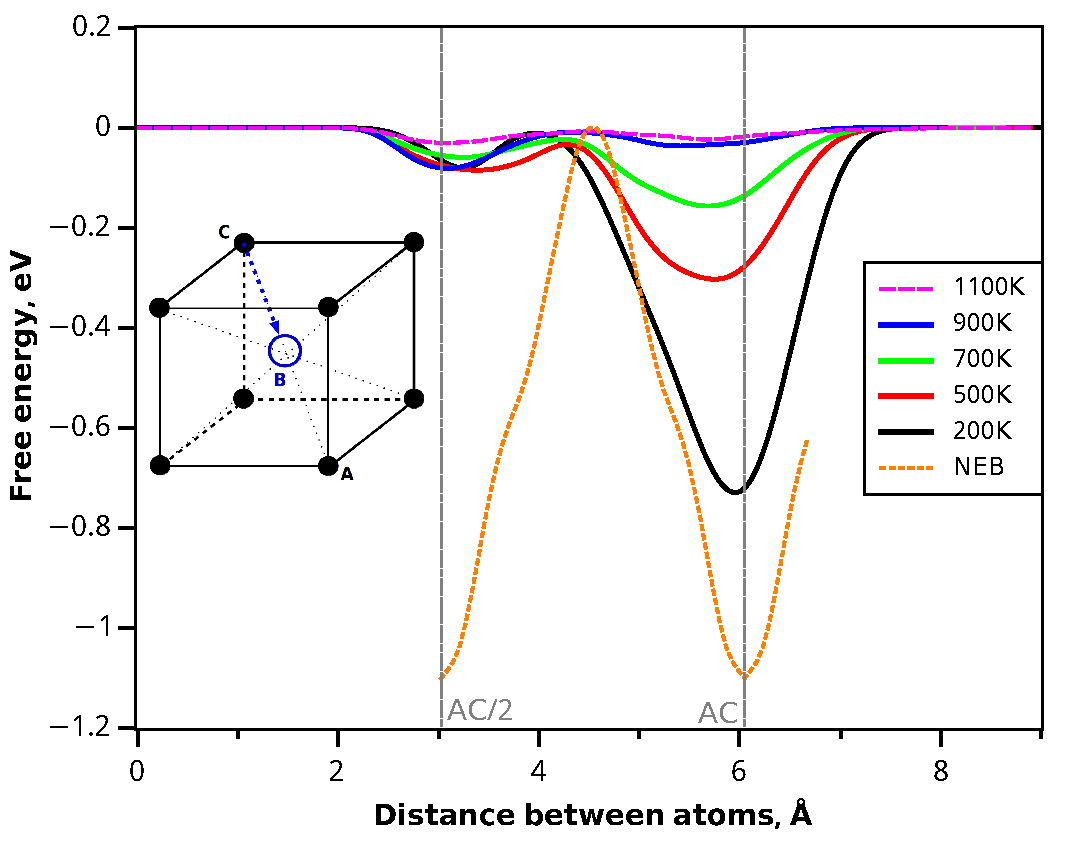
\includegraphics[width=.7\linewidth]{FES_(T).pdf}
\end{center}
%\caption{\label{graph_MetaD_FES} Free energy surfaces at different temperatures. All solid curves are averaged over 6-15 independent runs. The well at $AB/2$ is not visible, because the simulations were stopped after the jump of defect. Dashed orange curve shows the barrier $\Delta U$ obtained from NEB.}
\caption{\label{graph_MetaD_FES} Поверхности потенциальной энергии при разных температурах. Сплошные линии усреднены по 6-15 независимым расчетам. Потенциальная яма на $AB/2$ не видна, поскольку моделирование останавливалось сразу после скачка дефекта. Оранжевым пунктиром показан барьер $\Delta U$, полученный с помощью NEB.}
\end{figure}

%For consistency between the MSD data and metadynamics, the first ones were fitted by Arrhenius expression with temperature-dependent activation energy
Для сопоставления данных прямого МД-моделирования и метадинамики первые интерполировались аррениусовской кривой с энергией активации, зависящей от температуры:
\begin{equation}
D = a/2 \cdot \nu^\mathrm{NEB} \cdot \exp\left( - \frac{E_a(T)}{k_B T}\right).
\end{equation}
%Here $a/2$ is a geometric factor for $\left\langle 111\right\rangle$ jumps, $a$ is a lattice constant.
Здесь $a/2$ -- геометрический фактор для скачков вдоль $\left\langle 111\right\rangle$, $a$ -- постоянная решетки.
%The analytic form of $E_a(T)$ was obtained from the metadynamic data. This form is a topic for further discussion, but at current stage of research we simply use the exponential decrease
Аналитический вид $E_a(T)$ был получен из данных метадинамики. Эта форма представляет собой отдельный вопрос, но на данной стадии исследования мы просто используем экспоненциальный спад
\begin{equation}
E_a(T) = \Delta E^{\mathrm{NEB}} \cdot \exp{\left( -T/T_0\right)},
\end{equation} 
%as far as it gives good describing of metadynamic data. Here $T_0$ is a fitting parameter.
поскольку он дает хорошее описание данных метадинамики. Здесь $T_0$ -- свободный параметр.
\begin{figure}%[H]	% D(1/T) | W(T)
	\begin{center}
		\begin{minipage}{.7\linewidth}
			\begin{center}
				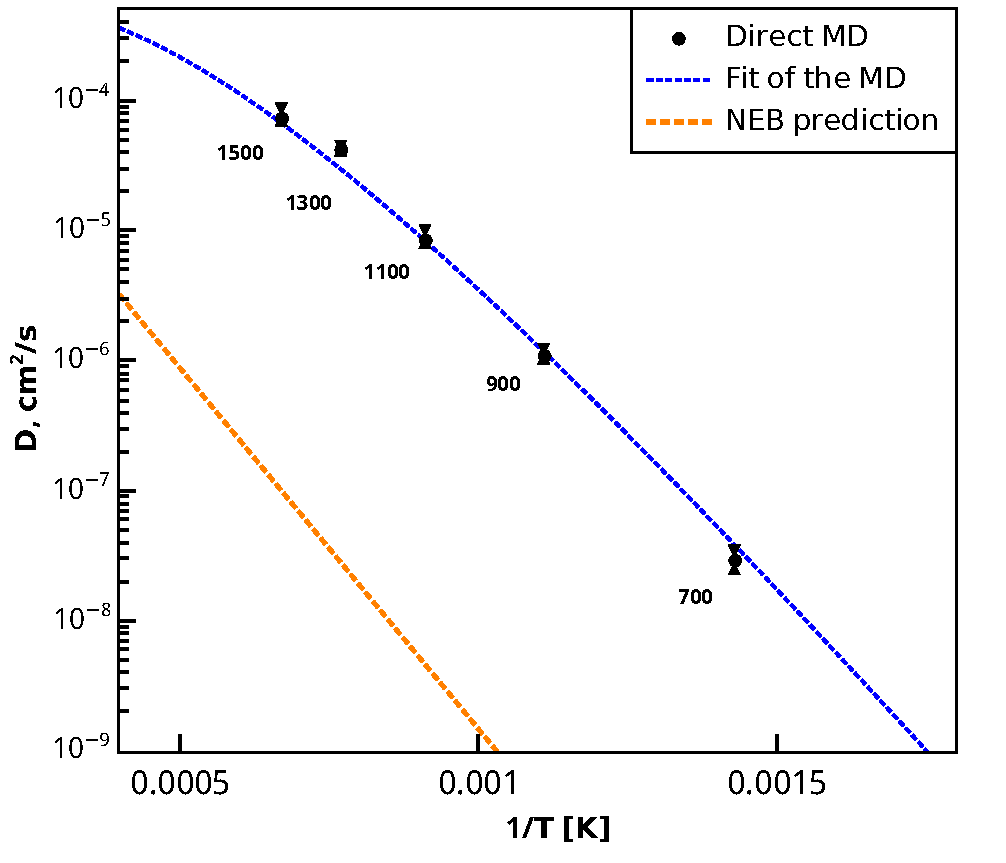
\includegraphics[width=1\linewidth]{D_1_T.pdf}

\textbf{a)}
			\end{center}
		\end{minipage} \hspace{1pc}
		\begin{minipage}{.7\linewidth}
			\begin{center}
				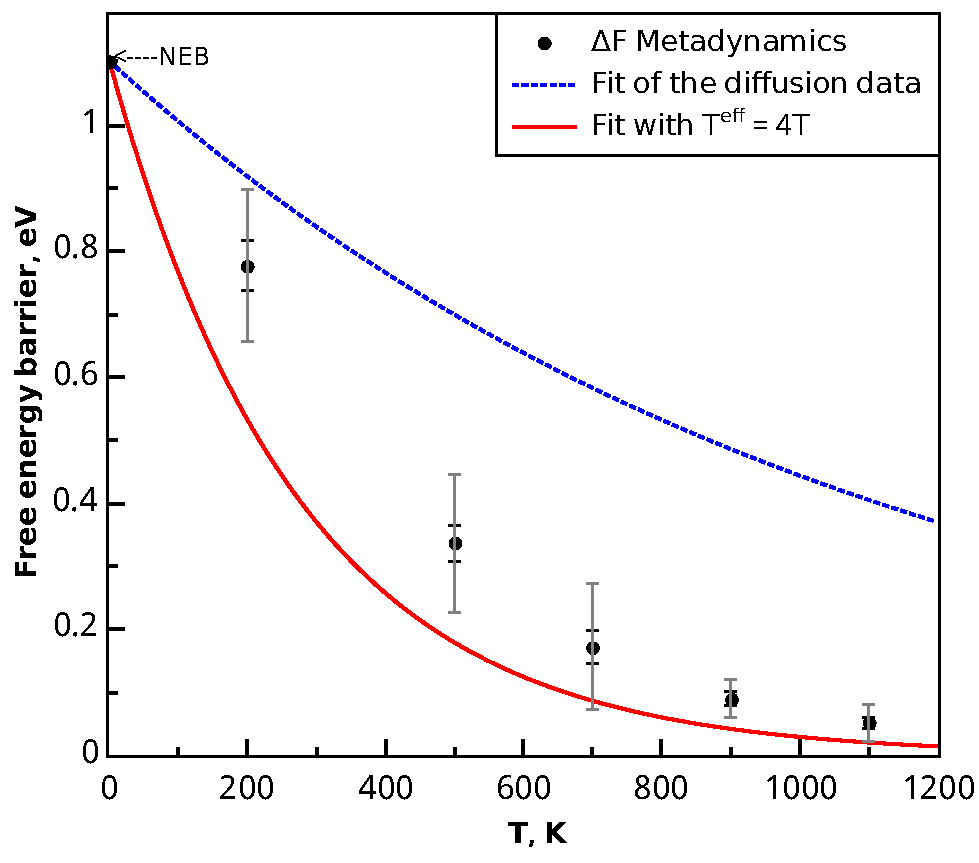
\includegraphics[width=1\linewidth]{W_T_metadynamics.pdf}

\textbf{b)}
			\end{center}
		\end{minipage}
	\end{center}

%\caption{\label{graph_MSD}a)Direct MD simulation of diffusion of vacancу. Orange line is a prediction from NEB barrier and frequency. b) Dependence of the metadynamic free energy barrier on temperature. Dashed blue line represents the $\Delta F(T)$ based on the direct MD simulation. Solid red line shows the same prediction, but with four times larger temperature $\Delta F(4T)$.}
\caption{\label{graph_MSD}a) Прямое МД-моделирование диффузии вакансии. b) Температурная зависимость барьера свободной энергии, полученная из метадинамики. Синий пунктир показывает $\Delta F(T)$, ожидаемый по данным прямого МД-моделирования. Красная сплошная линия показывает то же предсказание, но с увеличенной в 4 раза температурой $\Delta F(4T)$.}
\end{figure}
%When $T_0$ is obtained from MSD fit, it is moved back to figure~\ref{graph_MSD}b as dashed blue line. Although the trend is similar, we see noticeable discrepancy between the MSD prediction and metadynamic calculation of the barrier.
$T_0$, полученная из данных СКО, нанесена обратно на график~\ref{graph_MSD}b в виде синего пунктира. Хотя общий тренд похож, заметно сущетвенное расхождение между предсказанием из СКО и метадинамическими расчетами барьера.
%We interpret it as a specific feature of chosen collective variable. Since two oscillated atoms are involved in CV, relative velocity is twice higher, hence the effective temperature along this CV is 4 times higher. If we build $E_a(T)$ with $T^{\mathrm{ eff}} = 4T_0$ (solid red line at figure~\ref{graph_MSD}b), we see that measured values lie higher. It can be interpreted as interaction between CV and environing atoms with different effective temperature, so that resulting temperature effect lies between these two. At current stage this result is not accurate enough for applications, but the method seems to be promising for further development.
Мы интерпретируем это как специфическое свойство выбранной обобщеной координаты. Поскольку в нее входят координты двух атомов, относительная скорость их движения вдвое выше, следовательно, эффективная температура вдоль выбранной обобщенной координаты в 4 раза выше. Если мы построим $E_a(T)$ с $T^{\mathrm{ eff}} = 4T_0$ (красная линия на графике~\ref{graph_MSD}b), мы увидим, что измеренной значение лежит чуть выше. Это может быть интерпретировано как взаимодействие обобщенной координаты с окружением, так что итоговое значение лежит между этими двумя. На данном этапе этот результат недостотачно точен для практического применения, но метод выглядит многообещающим для дальнейшей разработки.

\section{Выводы}
%Serious difficulties in calculation of the Vineyard frequency for $\gamma$-U are shown. Due to instability of bcc lattice of U at zero temperature one cannot obtain normal frequencies. This problem doesn't occur for stable bcc-Mo. 
Показаны серьезные сложности в вычислении частоты Вайнъярда для $\gamma$-U. Из-за неустойчивости ОЦК-решетки урана при нулевой температуре невозожно получить спектр нормальных частот. Эта проблема не возникает в случае устоучивого ОЦК-Mo.

%Vibrational density of states for $\gamma$-U is calculated through the Fourier transform of velocity autocorrelation function. Significant temperature dependence of vDoS is a consequence of instability of the $\gamma$-U lattice at low temperature.
С помощью преобразования Фурье от автокоррелятора скорости построена плотность колебательных состояний для $\gamma$-U. Существенная температурная зависимость также является следствием нейстойчивости ОЦК-решетки при низких температурах.

%We suggest to use estimation of frequency factor from curvature of NEB potential surface instead of Vineyard frequency. Obtained frequency is much lower than maximum of vDoS, but there is an experimental evidence that this situation is typical for various bcc metals~\cite{BCC_Soft_Phonons}.
Предложен метод оценки предэкспоненты на основе кривизны потенциала NEB вместо расчета частоты Вайнъярда. Полученная частота много меньше, чем частота максимума распределения, но есть экспериментальное подтверждение, что такая ситуация характерна для различных ОЦК-металлов с высоким коэффициентом самодиффузии~\cite{BCC_Soft_Phonons}.

%Temperature dependence of free energy surface was obtained with metadynamic simulation. This dependence is significantly non-linear and gives the information about anharmonic contribution to the migration of vacancies. At low temperature metadynamics shows good agreement with the NEB results.
С помощью метадинамического моделирования получена температурная зависимость поверхности свободной энергии. Эта зависимость существенно нелинейна и дает информацию об ангармоническом вкладе в диффузию вакансий. На низких температурах показано хорошее согласие с результатами NEB.

%Calculation of diffusion coefficient for vacancies was carried out through calculation of MSD for the set of trajectories. At temperatures more than 1100 K diffusivity is lower than the Arrhenius equation predicts. This phenomena can be described in NEB+metadynamics framework, with the assumption that effective temperature along chosen collective variable in metadynamic simulation is more than measured temperature of whole system.
Через среднеквадратичное отклонение вакансии от начального положения на серии траекторий проведено вычисление коэффициента диффузии вакансий. На температурах больше 1100K коэффициент диффузии меньше, чем предсказывает закон Аррениуса. Этот факт может быть объяснен в контексте NEB+метадинамика, если сделать предположение, что эффективная температура вдоль выбранной в метадинамике обобщенной переменной больше, чем измеренная температура всей системы.
%Some questions about the form of $E_a(T)$ and accuracy of metadynamics remain, but they seem to be soluble.
Некоторые вопросы о форме $E_a(T)$ и точности метадинамичесих расчетов остаются, но они, вероятно, разрешимы.

\bibliography{Fidanyan_Spring_2016}
\bibliographystyle{gost705}

%\appendix
%\input{app-a}

\end{document}
